\documentclass[a4paper]{article}
\usepackage[margin=3cm]{geometry}
\usepackage{xcolor}
\usepackage{graphicx}
\usepackage{lipsum}
\usepackage{amsmath}
\usepackage{pdfpages}
\usepackage{url}
\usepackage{hyperref}
\usepackage{subcaption}
\hypersetup{
	colorlinks = true,
	colorlinks = false,
	linkbordercolor = {white},
	urlcolor = {blue},
	linkcolor = {blue},
	citecolor = {blue}
}
\usepackage{acronym}
\usepackage[acronym,nomain]{glossaries}
\makeglossaries
\newcommand{\todo}[1]{\textbf{\textcolor{red}{#1}}}
\newcommand{\td}[1]{\textbf{\textcolor{red}{#1}}}
\newcommand{\me}[1]{\textbf{\textcolor{gray}{#1}}}
\newcommand{\ds}[1]{}
\newcommand{\oc}{$^o$C}

\title{Functional oxide layers for electrical isolation and chemical passivation of steel substrates}
\author{Johann Dorn}

\begin{document}
\maketitle
\iffalse
my notes
\fi
%\begin{acronym}
%	\newacronym{nemo}{amat}{dolorem}
	\newacronym{zrpro}{Zr(PrO)$_4$}{zirconium(IV)propoxide}
	\newacronym{acac}{Hacac}{acetylacetone}
	\newacronym{acoh}{AcOH}{acetic acid}
	\newacronym{buoh}{BuOH}{1-buthanol}
	\newacronym{ipo}{IPO}{2-Propanol}
	\newacronym{ito}{ITO}{indium doped tin oxide}
	\newacronym{fto}{FTO}{fluorine doped tin oxide}
	\newacronym{n2}{N$_2$}{nitrogen}
	\newacronym{water}{H$_2$O}{deionized water}
	\newacronym{sds}{SDS}{sodium dodecyl sulfate}
	\newacronym{hcl}{HCl}{hydrochloric acid}
	\newacronym{h2so4}{H$_2$SO$_4$}{sulfuric acid}
	\newacronym{naoh}{NaOH}{sodium hydroxide}
	\newacronym{zro}{ZrO$_2$}{zirconium dioxide}
	\newacronym{1f}{1F}{one-fold concentrated solution}
	\newacronym{2f}{2F}{two-fold concentrated solution}
	\newacronym{3f}{3F}{three-fold concentrated solution}
	\newacronym{4f}{4F}{four-fold concentrated solution}
	\newacronym{5f}{5F}{five-fold concentrated solution}
	\newacronym{db}{DB}{doctor blading}
%\end{acronym}

\clearpage
\printglossaries
%\clearpage
%%%%%%%%%
%%%%%%%%%%%%%%%%%%%%%%%%%%%
%%%%%%%%%%%%%%%%%%%%%%%%%%%%%%%%%%%%%%%%%%%%%%%%%%%%%%
\section{Preface}
%%%%%%%%%
%%%%%%%%%%%%%%%%%%%%%%%%%%%
%%%%%%%%%%%%%%%%%%%%%%%%%%%%%%%%%%%%%%%%%%%%%%%%%%%%%%
\section{Introduction}
\td{describe everything what is meantioned in \ref{sec:exp}}
%%%%%%%%%
%%%%%%%%%%%%%%%%%%%%%%%%%%%
%%%%%%%%%%%%%%%%%%%%%%%%%%%%%%%%%%%%%%%%%%%%%%%%%%%%%%
\section{Aims and Objectives}
was hab ich gemacht, warum? 
Defensio: Argumente in der Arbeit noch mal sichten, Feedback von Betreuungsperson im Kopf haben - da könnten Fragen kommen, 
sich selbst aufnehmen 

Präsentieren: Visualisierungen sinnvoll? 
Antworten überlegen/Argumente überlegen
Limitation, Rahmen der Arbeit
Begründung für die eigene Vorgehensweise
%%%%%%%%%
%%%%%%%%%%%%%%%%%%%%%%%%%%%
%%%%%%%%%%%%%%%%%%%%%%%%%%%%%%%%%%%%%%%%%%%%%%%%%%%%%% EXPERIMENTAL
\section{Theoretical Background aka How does is work?}
\subsection{Sputtering}
\subsection{SEM}
\subsection{Infrared absorbance}

\section{Experimental}
\label{sec:exp}
In this section the used chemicals and substrates, experimental procedures and any used equipment are described. 
%%%%%%%%%%%%%%%%%%%%%%%%%%%
%%%%%%%%%%%%%%%%%%%%%%%%%%%%%%%%%%%%%%%%%%%%%%%%%%%%%%
\subsection{Substrate Preparation}
Five different substrates were used throughout this work: 
microscope glass slides (2.5~cm~x~7.5~cm) \td{from Sigma Aldrich}, thinner, squared glass plates (2.5~cm~x~2.5~cm) \td{from Sigma Aldrich}, \gls{ito} glass plates (2.5~cm~x 2.5~cm) \td{from Sigma Aldrich}, \gls{fto} glass plates (5~cm~x~5~cm) from \td{Sigma Aldrich} and steel foil (10~cm~x~10~cm) provided by Sunplugged GmbH (\url{http://sunplugged.at/)}.
The glass slides and \gls{fto} were \ds{cut\td{/scratched}}scratched with a scratching tool \ds{\td{(diamond scratcher/scraper)} }and broken with a \td{glass breaker} into pieces with dimensions 2.5~cm~x~2.5~cm.
The steel foil was cut with a foil cutter, a cutter knife (repeatedly), a paper cutter or a scissors (ordered by increasing curvature of resulting plates).
All substrates were cleaned in three steps before usage:
\begin{enumerate}
	\item 15 minutes in 50 ml \gls{water} and 1 ml of Hellmanex III in a sonic bath
	\item 15 minutes in \gls{water} in a sonic bath
	\item 15 minutes in \gls{ipo} in a sonic bath 
\end{enumerate}
After the last cleaning step, the samples were dry blown with dry \gls{n2} gas. 

%%%%%%%%%%%%%%%%%%%%%%%%%%%
%%%%%%%%%%%%%%%%%%%%%%%%%%%%%%%%%%%%%%%%%%%%%%%%%%%%%%
\iffalse
\subsection{Cutting of the steel foil}
\label{sec:cut}
There is a red foil cutter in the vacuum room, which cuts the foil without much bending.
Alternatively, the foil can be cut without bending by cutting repeatedly with a cutter knife.
The foil is cut into 2.5 x 2.7 mm plates.
The small plates are marked with an diamond cutter pen.
The plates are cleaned with 1ml of Hellmanex III in 50-100 ml \gls{water} in the sonic bath for 15 min, then in \gls{water} for 15 min and finally in \gls{ipo} for 15 min. 
The samples are dry blown with dry N$_2$ and stored until doctor blading.
\fi
%%%%%%%%%%%%%%%%%%%%%%%%%%%
%%%%%%%%%%%%%%%%%%%%%%%%%%%%%%%%%%%%%%%%%%%%%%%%%%%%%%
\subsection{Solution}
Two main recipes were used and their compositions were varied. 
The first recipe - adopted from Anwar et. al. \cite{Anwar2017} - was based on \gls{zrpro} in \gls{acac} and \gls{water} 
and the second recipe - 
adopted from Hu et. al. \cite{Hu2016} -
was based on \gls{zrpro} in \gls{buoh}.

%\iffalse
\begin{figure}[htb]
	\centering
	\begin{subfigure}{0.49\textwidth}
		\centering
		%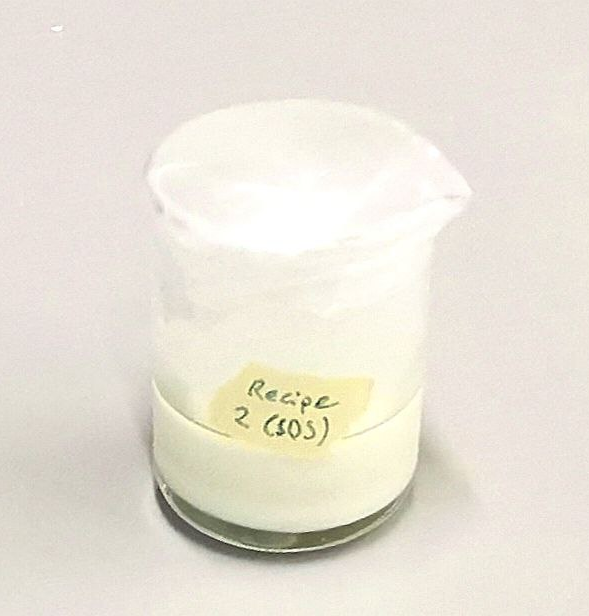
\includegraphics[width=.99\textwidth]{Pics/sol-aq.png}
		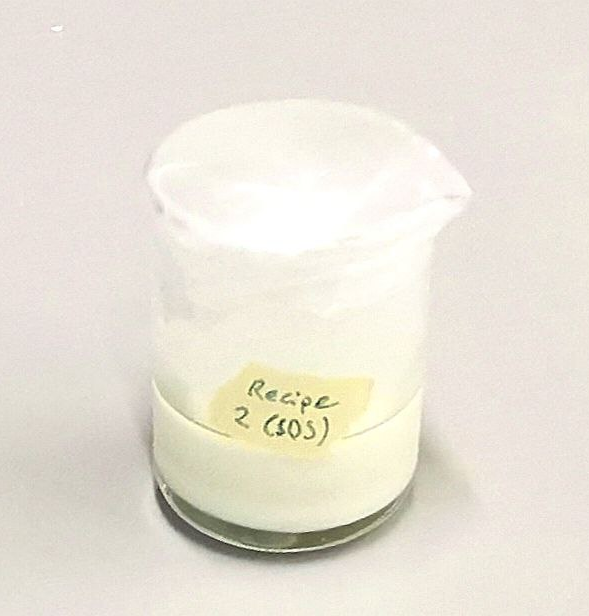
\includegraphics[height=0.8\textwidth]{Pics/sol-aq.png}
		\label{fig:sol-aq}
		\caption{Aquatic solution}
	\end{subfigure}
	\begin{subfigure}{0.49\textwidth}
		\centering
		%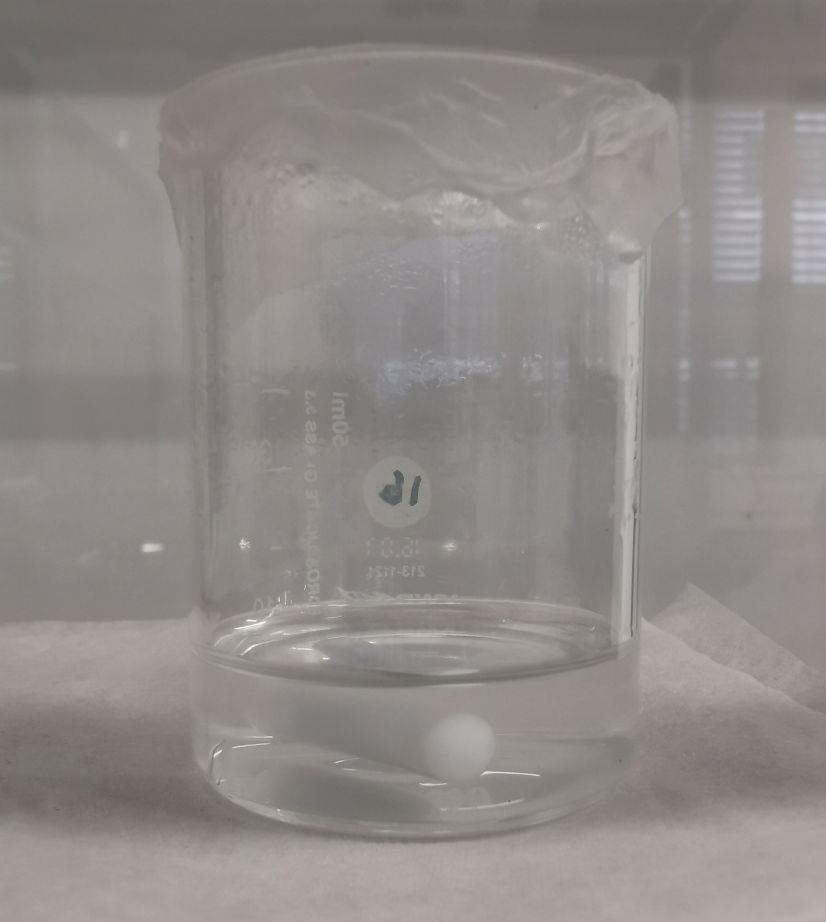
\includegraphics[width=.99\textwidth]{Pics/sol-bu.png}
		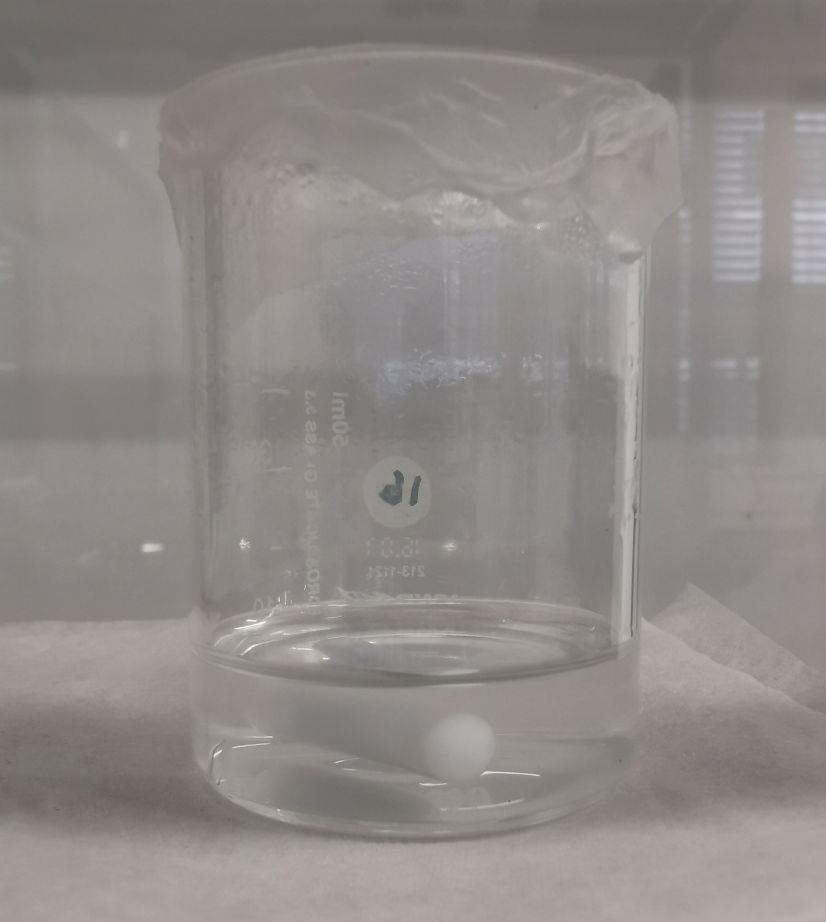
\includegraphics[height=0.8\textwidth]{Pics/sol-bu.png}
		\label{fig:sol-bu}
		\caption{Buthanolic solution}
	\end{subfigure}
	\label{fig:sol}
	\caption{Aquatic and buthanolic solution in beaker glass sealed with Parafilm}
\end{figure}
%\fi

%%%%%%%%%%%%%%%%%%%%%%%%%%%%%%%%%%%%%%%%%%%%%%%%%%%%%%
\subsubsection{Aquatic solution}
\me{The procedure for the aquatic solution is as follows:}
\gls{zrpro} was added to \gls{acac} while stirring and in a seperate vessel \gls{water} (including any additives such as \gls{sds}, \gls{hcl}, \gls{h2so4} or \gls{naoh}) was added to \gls{ipo} and both were stirred for 1 hour. 
The \gls{water}-\gls{ipo} mixture was added to the other solution and stirred over night. 
The exact volumes can be taken from table \ref{tab:rec1}.
\begin{table}[h]
	\centering
	\caption{}
	\label{tab:rec1}
	\begin{tabular}{llllllll}
		\hline
		recipe				&1		&2		&3		&4		&5		&6		&7\\
%		\hline
%		conc. [a.u.]	&1		&1.7	&2.6	&3.5	&4.4	\\
		\hline
		\gls{zrpro} [ml]	&8		&8		&8		&8		&8		&8		&8\\
		\gls{acac} [ml]		&8		&8		&8		&8		&8		&8		&8\\
		\gls{ipo} [ml]		&2		&2		&2		&2		&2		&2		&2\\
		\gls{water} [ml]		&2.6	&2.6	&2.5	&2		&2		&2		&2\\
		\gls{sds} [mg]		&-		&5.9	&-		&-		&-		&-		&-\\
		\gls{hcl} [ml]		&-		&-		&-		&-		&0.5	&-		&-\\
		\gls{h2so4} [ml]	&-		&-		&-		&-		&-		&0.5	&-\\
		\gls{naoh} [ml] 	&-		&-		&-		&-		&-		&-		&0.5\\
		\hline
	\end{tabular}
\end{table}
%
%%%%%%%%%%%%%%%%%%%%%%%%%%%%%%%%%%%%%%%%%%%%%%%%%%%%%%
\subsubsection{Buthanolic solution}
\label{sec:sol}
Five different concentration were prepared. 
%The first solution \td{(standard concentration/ one fold/ 1F)} 
%followed the recipe loosely, which is described by Hu et al. \cite{Hu2016}.
%In order to obtain thicker \gls{zro} layers the \gls{zrpro} concentration in the starting solution was raised.
The \gls{1f} 
was closest to the recipe proposed by Hu et. al. \cite{Hu2016}. 
The other four solutions (\gls{2f}, \gls{3f}, \gls{4f}, \gls{5f}) were similar with higher concentrations of \gls{zrpro} (see table \ref{tab:rec2}).
%%%%%%%%%%%%%%%%%%%%%%%%%%%%%%%%%%%%%%%%
\iffalse
The procedure for obtaining the \gls{1f} solution will be explained in detail: \td{maybe just keep it general}
%
%was closely on the basis of ref \cite{Hu2016}. 
%The standard concentration will be described first and then the differences of higher concentrated solutions:
4.9 ml of solvent (\gls{buoh}) are put into a beaker glass (or similar, preferably with an air-tight cap) with a stirrer. 
0.1 ml of \gls{zrpro} are added while stirring.  
After 10 to 15 minutes 0.05 ml (\ds{approximately }one mole equivalent of \gls{zrpro}) chelating agent (\gls{acac}) is added and stirred for another 10 to 15 minutes. 
Finally, 1 ml of stabilisation solvent (\gls{ipo} or \gls{acoh}) is added to the mixture and stirred for additional 20-30 minutes. 
\fi
%%%%%%%%%%%%%%%%%%%%%%%%%%%%%%%%%%%%%%%%
The solvent (\gls{buoh}) is put into a beaker glass (or similar, preferably with an air-tight cap) with a stirrer and \gls{zrpro} is added while stirring.  
After stirring 10 to 15 minutes one mole equivalent chelating agent (\gls{acac}) is added and stirred for another 10 to 15 minutes. 
Finally, the stabilisation solvent\cite{Hu2016} (\gls{ipo} or \gls{acoh}) is added to the mixture and stirred for additional 20-30 minutes. 
Following stirring times (in minutes) were tested and didn't have an influence on stability of the solution: 10-10-20, 10-10-45, 30-30-180. 
%%%%%%%%%%%%%%%%%%%%%%%%%%%%%%%%%%%%%%%%
In order to make a \gls{2f} solution, the volume of \gls{zrpro} and \gls{acac} is doubled and \gls{buoh} is decreased by the volume of \gls{zrpro}. 
The real concentration of a \gls{2f} solution is not double of the original, though, but rather 1.7 fold because volume of \gls{ipo} is kept constant.

\begin{table}[h]
	\centering
	\caption{}
	\label{tab:rec2}
	\begin{tabular}{rlllll}
		\hline
				&1F		&2F		&3F		&4F		&5F		\\
		\hline
		conc. [a.u.]	&1		&1.7	&2.6	&3.5	&4.4	\\
		\hline
		\gls{buoh} [ml]		&4.95	&4.9	&4.85	&4.8	&4.75	\\
		\gls{zrpro} [ml]	&0.05	&0.1	&0.15	&0.2	&0.25	\\
		\gls{acac} [ml]		&0.0125	&0.025	&0.0375	&0.05	&0.0625	\\
		\gls{ipo}/\gls{acoh} [ml]		&2		&2		&2		&2		&2		\\
		\hline
	\end{tabular}
\end{table}

\subsection{Doctor blading}
\label{sec:DB}
\begin{figure}
	\centering
	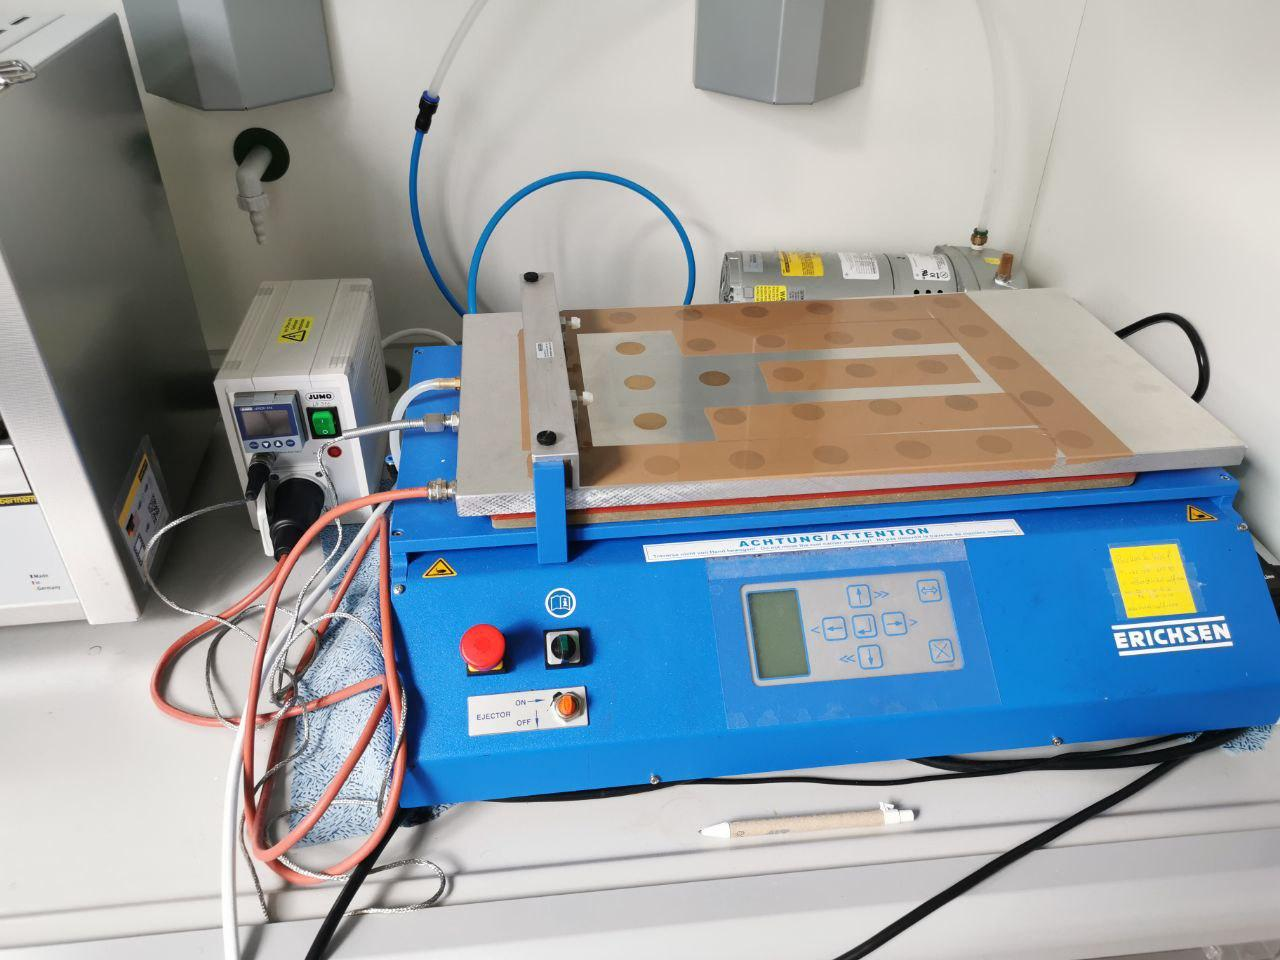
\includegraphics[width=.8\textwidth]{Pics/erichsen.png}
	\caption{Erichsen Coatmaster 510 
		%Doctor blading machine 
		with vacuum pump in the background and temperature regulator on the left.}
	\label{fig:eric}
\end{figure}
\td{picture of the machine, and name of the machine}
The temperature of the heating plate is set to 200 $^o$C.
The temperature of the vacuum plate is set and waited until reached.
The sample is placed on the vacuum plate and tested if it can be \td{held/retained} by the underpressure.
The velocity of the \gls{db} blade is set and a mini test run is performed. 
The blade is put in position. 
100-125 $\mu$l of solution is applied with an 10-1000 $\mu$l pipette and the doctor blading is started immediately. 
After evaporation of the solution, the vacuum is turned of, the 'blade pusher' put into initial position, the blade removed and excess solution removed with a wipe. 
The small metal plate is transferred to the hot heating plate and rests on there for 3-5 min. 
The process is repeated as wished. 

\subsection{Calcination}
A LabTech EH45 C heating plate and a Naberterm \td{L B410} furnace were used to calcinate the doctor bladed samples. 
The heating plate heated with a steady rate of \td{2} $^o$C/min. 
In order to achieve a lower overall heating rate several temperature ramps and plateaus were \todo{used}. See table~\ref{tab:labtech}


\begin{table}[h]
	\centering
	\begin{tabular}{rl ll ll ll ll ll ll }%ll ll ll ll ll ll ll}
%			&temp [\oc]	&time/rate &temp [\oc]	&time/rate	&temp [\oc]\\
		HP1		&&&&&&&&&&&&&\\
		\hline
		T [\oc]	&80		&100	&150	&160	&170 	&180	&190	&200	&250	&300	&350	&400	\\
		t [min]	&10 	&10		&5 		&5 		&5 		&5 &5 &10 &10 &10 &10 &60 \\
		\hline
	\end{tabular}
	\caption{Time the temperature was held constant at certain temperatures on the heatingplate}
	\label{tab:labtech}
\end{table}


\begin{table}[h]
	\centering
	\begin{tabular}{rl ll ll}% ll ll ll ll }%ll ll ll ll ll ll ll}
%			&temp [\oc]	&time/rate &temp [\oc]	&time/rate	&temp [\oc]\\
		HP1		&&&&&\\%&&&&&&&&\\
		\hline
		T [\oc]				&80		&150	&200	&400	&400 	\\
		$\theta$ [\oc/min]	&10 	&10		&5 		&5		& 		\\
		\hline
		name	&80-150 [\oc/min]	&150-200 [\oc/min]	&200-T$_{max}$ [\oc/min]	&T$_{max}$ [min]	&T$_{max}$ [\oc] \\
		NT1		&2					&1					&2					&60 &400 \\
		NT2		&2					&2					&2					&60 &400 \\
		NT3		&3					&3					&3					&60 &400 \\
		NT4		&4					&4					&4					&60 &400 \\
		NT5		&4					&4					&4					&60 &500 \\
		NT6		&1					&1					&1					&60 &400 \\
		NT7		&max				&max				&max				&60 &600 \\
		\hline
	\end{tabular}
	\caption{Heating rates and constant temperature times. \td{Macht dieser Graph ueberhaupt sinn? }}
	\label{tab:nt}
\end{table}

\subsection{Characterisation}
\subsubsection{SEM}
Zeiss Supra 40
\subsubsection{Infrared}
Bruker Vertex 70
\subsubsection{X-Ray Defraction}
Thermo Scientific ARL Equinox 100 X-Ray Diffractometer
\subsubsection{Current-Voltage Curve}
Agilent 4156C Precision Semiconductor Parameter Analyzer
\begin{figure}
	\centering
	\begin{subfigure}{0.48\textwidth}
		\centering
		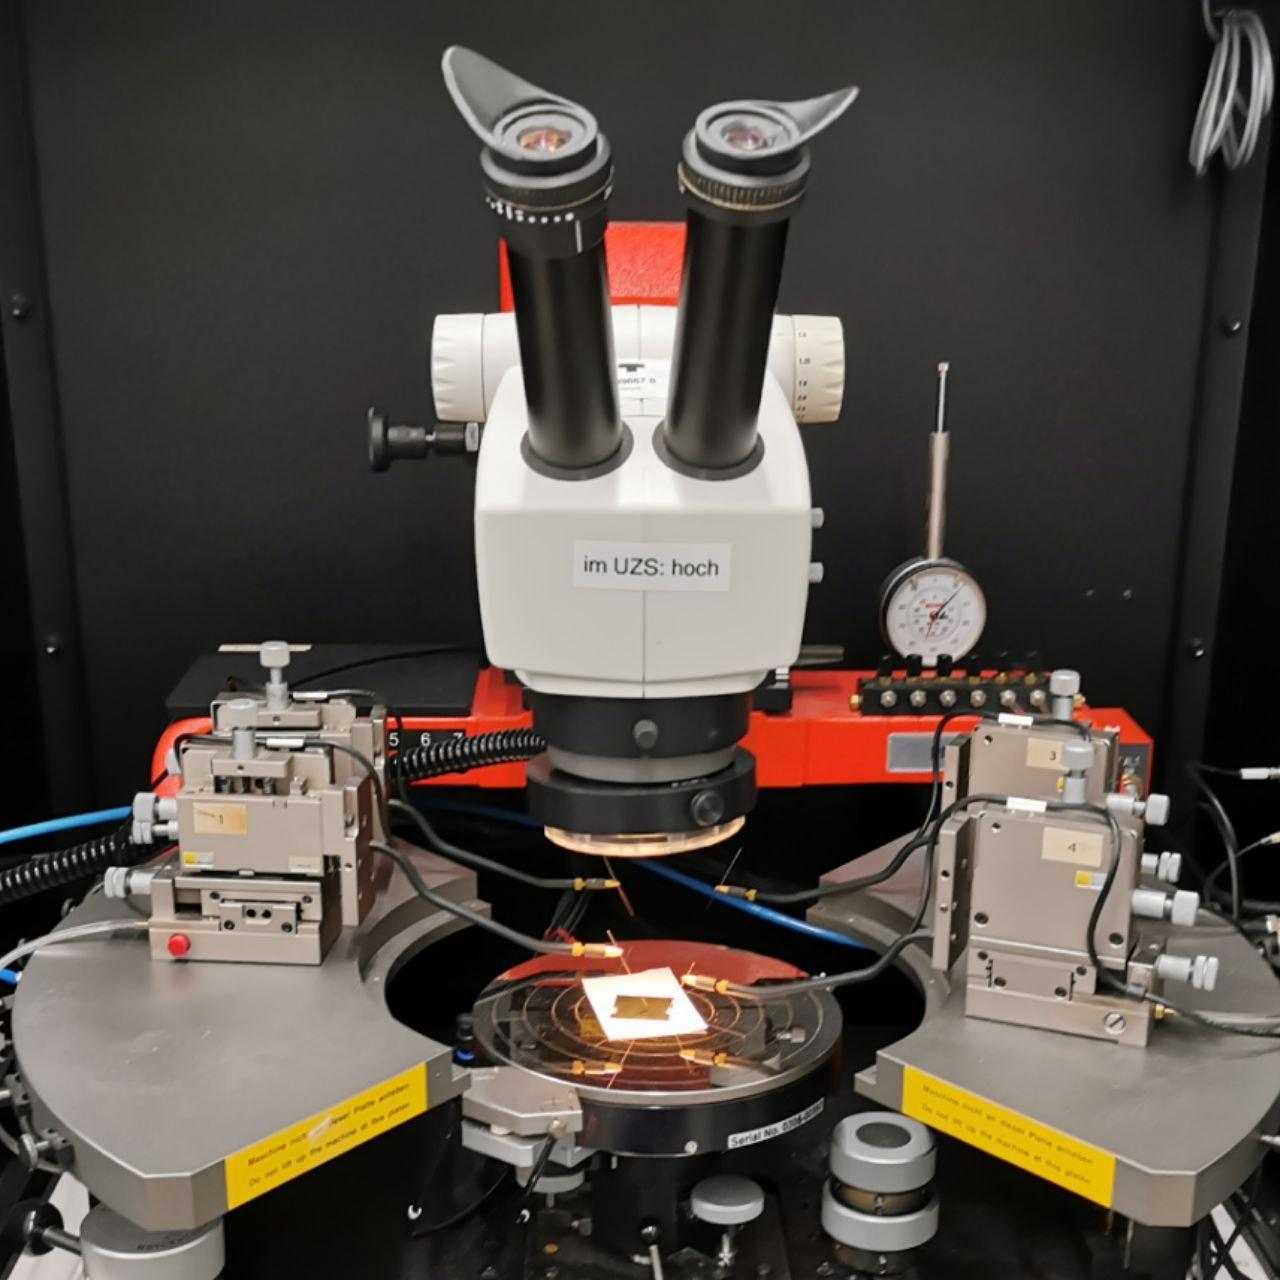
\includegraphics[width=.9\textwidth]{Pics/i-v.png}
		\label{fig:iv-agilent}
		\caption{peripherals}
	\end{subfigure}
	\begin{subfigure}{0.48\textwidth}
		\centering
		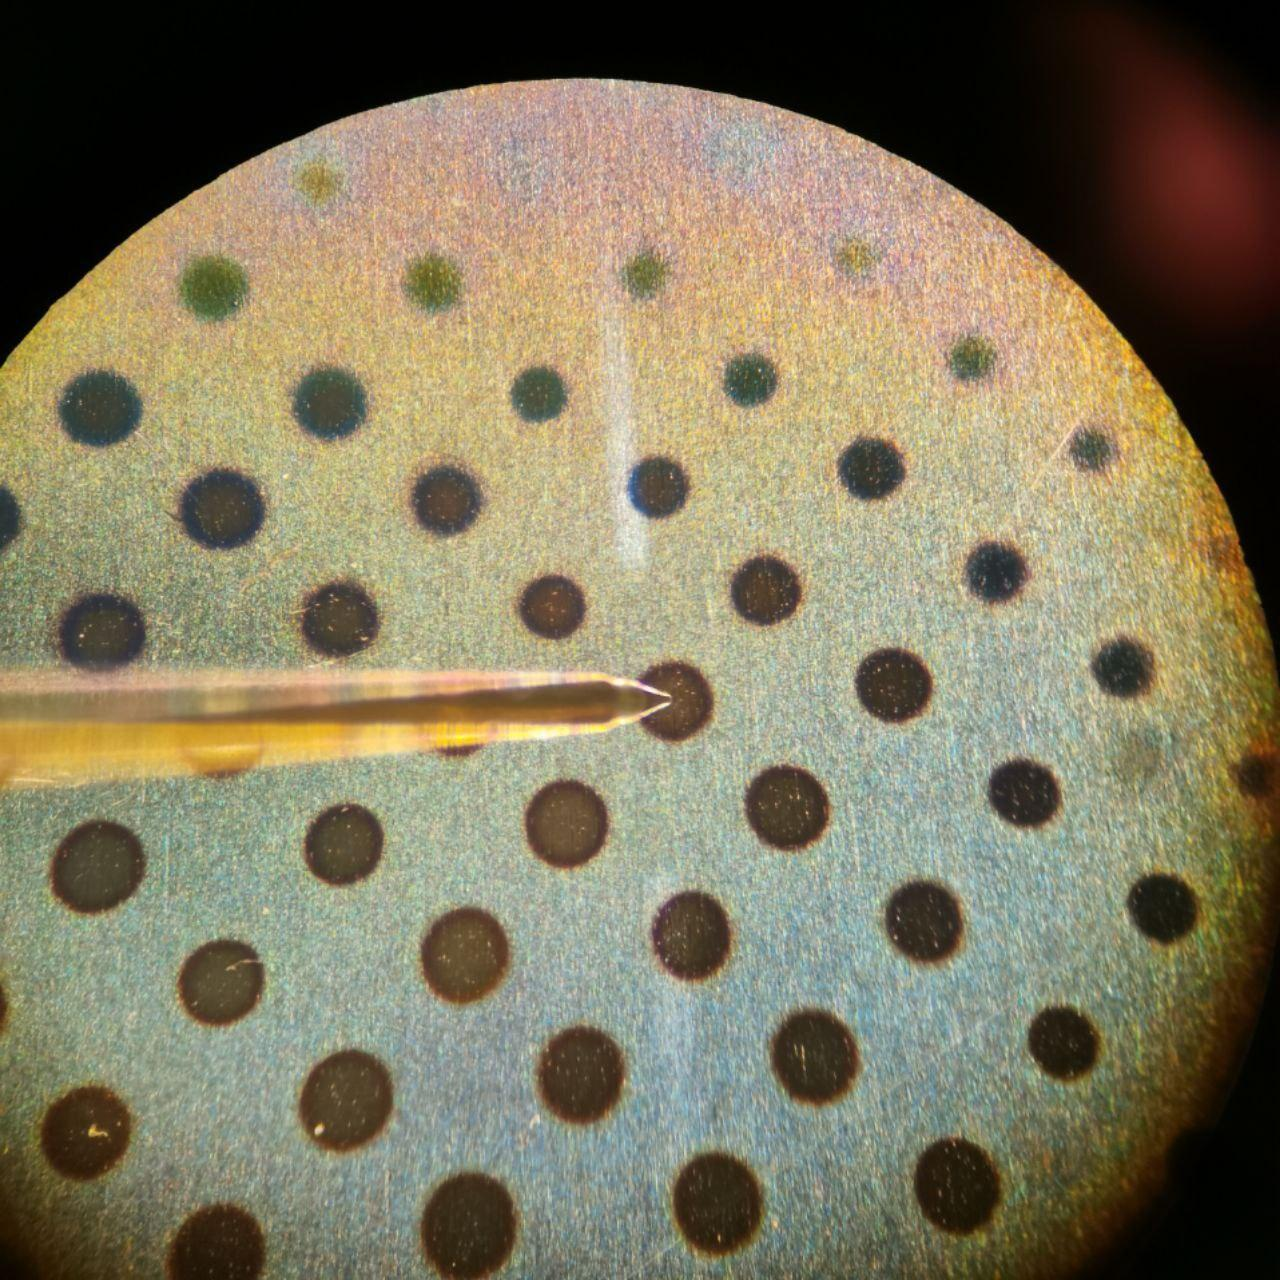
\includegraphics[width=.9\textwidth]{Pics/i-v-micro.png}
		\label{fig:iv-micro}
		\caption{View through the microscope}
	\end{subfigure}
	\label{fig:iv}
	\caption{I-V curve abnehm aperature and sicht durch das micro scope.}
\end{figure}


\subsection{EMMA Propagation}
\begin{table}
	\centering
	\begin{tabular}{ccccccc}
		\hline
		\hline
conc	&layers	&vDOC	&TDOC	&vCal	&Tcal	&	\\
		\hline
1	&10	&5	&20	&120	&400	&\\
1	&4	&0.1	&20	&120	&500	&\\
5	&10	&0.1	&20	&120	&500	&\\
5	&4	&5	&20	&480	&400	&\\
1	&5	&5	&80	&120	&500	&\\
1	&10	&1	&80	&480	&400	&\\
5	&5	&1	&80	&120	&400	&\\
5	&10	&5	&80	&480	&500	&\\
2	&8	&0.5	&40	&360	&470	&\\
2	&6	&2	&40	&360	&430	&\\
		\hline
%4	&12	&-	&-	&-	&-&\\
1	&4	&12	&70	&120	&500	&\\
1	&9	&18	&80	&240	&400	&\\
%2	&5	&18	&70	&-	&-		&\\
4	&6	&14	&60	&240	&500	&\\
4	&6	&14	&60	&240	&500	&\\
4	&6	&14	&60	&240	&500	&\\
		\hline
2	&10	&20	&40	&120	&500	&6113\\
3	&8	&18	&70	&1080	&300	&2850\\
3	&6	&10	&50	&1080	&400	&5526	\\
%3	&10	&14	&50	&600	&500	&-7374	\\
3	&10	&16	&80	&120	&500	&6554	\\
4	&6	&16	&80	&1080	&300	&2947	\\
3	&12	&12	&80	&840	&500	&8318	\\
3	&10	&14	&50	&600	&500	&7374	\\
5	&6	&10	&60	&1080	&400	&5648	\\
5	&10	&20	&60	&360	&300	&3956	\\
5	&12	&14	&60	&1080	&300	&2700	\\
		\hline
%2	&2	&10	&40	&600	&300	&-7201	\\
2	&4	&10	&80	&1080	&300	&6101	\\
%2	&4	&10	&40	&600	&300	&-7201	\\
2	&4	&10	&40	&600	&300	&7201	\\
3	&4	&12	&60	&600	&300	&1462	\\
4	&4	&10	&80	&1080	&300	&2883	\\
5	&12	&20	&70	&600	&300	&1680	\\
		\hline
2	&4	&10	&40	&120	&300	&1	\\
2	&4	&10	&40	&120	&500	&6001	\\
3	&4	&10	&40	&120	&500	&6102	\\
5	&4	&10	&80	&1080	&300	&2884	\\
5	&12	&20	&60	&120	&300	&360	\\
		\hline
3	&4	&10	&40	&600	&400	&4202	\\
2	&6	&20	&40	&120	&500	&6105	\\
%4	&4	&14	&80	&1080	&300	&-2923	\\
5	&12	&14	&60	&600	&300	&1500	\\
3	&6	&14	&60	&600	&300	&1486	\\
4	&4	&14	&80	&1080	&300	&2923	\\
		\hline
4	&8	&18	&80	&1080	&300	&2971	\\
3	&8	&10	&50	&1080	&300	&2530	\\
2	&12	&16	&40	&120	&400	&3077	\\
2	&10	&18	&60	&1080	&300	&2733	\\
4	&10	&10	&50	&1080	&300	&2535	\\
		\hline
		\hline
	\end{tabular}
	\caption{}
	\label{tab:emma}
\end{table}


\section{Evaluation and Computational Details}
\subsection{Evaluation of Samples}
\label{sec:eval}
For every I-V curve (aluminium dot) the gradient $g$ at V=0 is calculated by taking 5 points after the origin and 5 points before the origin, averaging their V and I values and calculating i
\begin{equation}
	g = \frac{I_{n+1} - I_n}{V_{n+1} - V_n}.
\end{equation}
As a measure of conductance a distance D from an ideal non-conducting case. The average of the negative base 10 logarithm subtracted from an ideal non-conducting gradient of $10^{-13}$ 
\begin{equation}
	D = \sum_i^N \frac{ -log_{10}(g_i) - 13}{N}
	\label{eq:D}
\end{equation}
Another measure is the density of shorted species $\rho_{s}$ is calculated in following way:
\begin{equation}
	s_i = \begin{cases}
	1 &\text{if} \quad -log(g_i) < 5 \\
	0 &\text{if} \quad -log(g_i) \geq 5 \\
	\end{cases}
\end{equation}
\begin{equation}
	\rho_s = \sum_i^N \frac{s_i}{N}
	\label{eq:rho}
\end{equation}
Other estimates of the conductance are the averages:
\begin{equation}
	G_1 = log \left( \sum_i^N \frac{g_i}{N} \right)
\end{equation}

\begin{equation}
	G_2 =  \sum_i^N \frac{log(g_i)}{N}
\end{equation}

\subsection{Sample Selection}
\label{sec:ss}
An evolutionary approach was chosen, namely a multi-objective Particle Swarm Optimization (PSO) with a multi-response
Multivariate Adaptive Regression Splines (MARS) model\cite{Villanova2010,Kennedy1995,Breiman1997,Carta2011}.
%
"PSO is a population based heuristic inspired by the flocking behavior of birds. 
To simulate the behavior of a swarm, each bird (or particle) is allowed to fly towards the optimum solution."\cite{Villanova2010}
%
Initially the input parameters (independent variables), their boundaries and number of equidistant levels for each parameter are declared (see table \ref{tab:input}).
Next, the output variables (dependant variables), their weights in the objective function (the function which should be optimized) are specified and if they should be minimized or maximized is noted.
%
%An initial population of particles, i.e. experiments with certain parameters, is chosen out of the population space (space spanned by all possible combinations of input parameters), 
\begin{table}[htb]
	\centering
	\begin{tabular}{cc cc cc}
		\hline
		Zr(PrO)$_4$ conc. [21 g/L]	&layers	&$T_{DB}$[$^o$C]	&$v_{DB}$[mm/s]	&$T_{cal}$[$^o$C]	&$v_{cal}$[$^o$C/hour]	\\
		\hline
		2				&4		&40					&10				&300				&120	\\
		3				&6		&50					&12				&400				&360	\\
		4				&8		&60					&14				&500				&600	\\
		5				&10		&70					&16				&					&840	\\
						&12		&80					&18				&					&1080	\\
						&		&					&20				&					&		\\
		\hline
	\end{tabular}
	\caption{Discrete levels of each input parameter \td{are concentrations correct?}}
	\label{tab:input}
\end{table}

The first step is to select an initial population (ensemble of experiments), which is chosen randomly from the population space. 
The samples are made, measured and evaluated according to section \ref{sec:exp} and the distance $D$ (see eq. \ref{eq:D}), $\rho_s$ (see eq. \ref{eq:rho}), $n_{layers}$ (numbers of layers) and $v_{cal}$ (heating rate of calcination process in $^o$C/min) are supplied to the program. 
The program uses this data to estimate a response for each output variable (and to choose a fraction of the initial population which is allowed to propagate).
The response variables for the entire population space is calculated. 
The current population - each of the particles independently - moves towards the optimum solution.
The population for the next time step is outputted and the experiments are again executed, measured and evaluated.


scarce data may lead to overfitting\cite{Lecun1995conv}
\section{Results and Discussion}
The space seems to be too big for the small sample size.
Look at relation of space size and sample size here and in Hu2016.

Would be easier to fit with single factor at a time variation or latin hyper cuber?
Would it also be easier for PSO or ML to find fitting function?
Every output var is independent of each other, so $v_{cal}$ can act as test 

\section{Outlook}

Making of the solution for the sol-gel process:
For a single concentrated solution 0.05 ml of \gls{zrpro} are added while stirring to 4.95 ml of \gls{buoh} and stirred for 15 minutes. 
0.013 ml (or one molar equvilent of Zr) of \gls{acac} is added to the stirring solution. 
After another 15 minutes 1 ml of acetic acid is added and stirred for 30 minutes to stabilize the solution up to 24h. 

The concentration can be increased up to 5 times being stable for a minimum of 4 hours. 
The sol-gel process produces am homogeneous transparent crystalline zirconia oxide layer. 
homogeneity can be mainly controlled via blade velocity and temperature and layers can be stacked.

%\clearpage
\bibliographystyle{ieeetr}
\bibliography{int}
\end{document}
